\documentclass {article}
\usepackage{amsmath}
\setlength{\parindent}{0cm}

\usepackage{hyperref}
\usepackage{graphicx}
\usepackage{subcaption}
\usepackage[margin=1.5in]{geometry}
\usepackage{tikz}			% for graphs
\usepackage{float}			% for having the graphs not fly off into space
\usetikzlibrary{arrows}

\usepackage{fancyhdr}
\pagestyle{fancy}
\lhead{\textbf{Complex Network Analysis} \\ Assignment 3\\}
\rhead{Maria Kagkeli \\ Maria Regina Lily \\ Mihai Verzan}
\headheight 10pc
\voffset -10pc

\begin{document}



% problem 1
\section{Power Laws}

\subsection{}
(a) $ \to $ not scale-free, because the plot is curved, therefore $ \log p_k $ does not depend linearly on $ \log k $.

(b) $ \to $ scale-free, because $ \log p_k $ depends linearly on $ \log k $ (the plot is approximately a straight line).

\subsection{}
$ \log_{10} p_k \sim - \gamma \cdot log_{10} k \Rightarrow
  \gamma = - \frac{ \log_{10} p_k }{ \log_{10} k } $. 
Sample several points on the graph and estimate the values in those points, then plug them in the formula:

\begin{itemize}
  \item $ k = 10 $, $ p_k = 10^{-2} \Rightarrow \gamma = 2 $
  \item $ k = 2  $, $ p_k = 10^{-1} \Rightarrow \gamma = 3.321 $
  \item $ k = 50 $, $ p_k = 10^{-3} \Rightarrow \gamma = 1.765 $
\end{itemize}

We can estimate $ \gamma $ to be around 2.

\subsection{}
$ \gamma = 1 + N[\sum^N_{i=1} \ln \frac{ K_i }{ K_{min}-\frac{1}{2} }] = 1.756 $, $ \sigma = 0.16913 $ (values calculated using a Python script. See 4-1.ipynb).

\newpage



% problem 2
\section{Configuration Model}

\subsection{}
$ k = (4, 1, 1) $: One node has degree 4, yet there are only 3 nodes in total. This is impossible without forming self-loops or multiple edges.

\subsection{}
$ k = (3, 2, 1, 1, 1) $:
\begin{figure}[H]
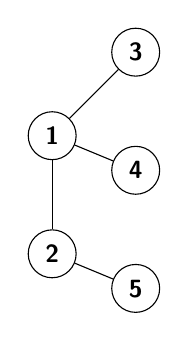
\begin{tikzpicture}[auto,node distance=1.5cm,
                    thin,main node/.style={circle,draw,font=\sffamily\small\bfseries}]
  \node[main node] (1) {1};
  \node[main node] (2) [below of=1] {2};
  \node[main node] (3) [above right of=1] {3};
  \node[main node] (4) [below of=3] {4};
  \node[main node] (5) [below of=4] {5};

  \path[every node/.style={font=\sffamily\small}]
    (1) edge node [left] {} (3)
        edge node [left] {} (4)
        edge node [left] {} (2)
    (2) edge node [right] {} (5);
\end{tikzpicture}
\end{figure}

\subsection{}
$ k = (3, 3, 1, 1) $:
Impossible. There are 4 nodes, and 2 of them have degree 3. Therefore, both of these two nodes would each have to be connected to all 3 others respectively, so the remaining two nodes must have at least degree 2, which is not the case.

\end{document}